\section{Theorie}
\label{sec:Theorie}

Ziel des Versuches ist die Bestimmung der Materialien und Strukturen
metallener Würfel. Dazu soll die Gammastrahlentomographie als
bildgebendes Verfahren zur schichtweisen Darstellung der Proben
angewandt werden und Erkenntnisse über die Licht-Materie-Wechselwirkung liefern.\\

Praktisch wird die Absorption der Strahlung für verschiedene
Schnittgeometrien untersucht, indem die Intensität transmittierter
Strahlung

\vspace{-5pt}
\begin{equation}
    I = I_0 \cdot \text{exp}\left(- \sum_i \mu_i d_i \right)
    \label{eqn:int}
\end{equation}

gemessen wird. Diese hängt von den Dicken $d_i$ und Absorptionskoeffizienten $\mu_i$
der $i$ verschiedenen durchstrahlten Materialien ab.
Schnittmessungen einer Substruktur aus verschiedenen Winkeln ergeben Projektionen
die dann zu einer Zweidimensionalen Darstellung der gesamten Struktur zusammengesetzt
werden können.

Als Strahlungquelle wird in diesem Versuch $\ce{^{137}Cs}$ verwendet. Das zugehörige 
Zerfallsschema mit dem Endprodukt $\ce{^{137}Ba}$ ist in Abbildung \ref{fig:schema}
dargestellt. Wie daraus zu entnehmen ist, zerfällt $\ce{^{137}Cs}$ über den $\beta^{-}$-Zerfall nur zu etwa $\SI{6.5}{\percent}$
in $\ce{^{137}Ba}$ im Grundzustand und zu $\SI{93.5}{\percent}$ in $\ce{^{137}Ba}$ im angeregten Zustand.
Der Übergang des angeregten Zustandes in den Grundzustand erfolgt schließlich unter Emission von
Gammaquanten der Energie von etwa $\SI{662}{\kilo\eV}$.

\vspace{-15pt}
\begin{figure}
    \centering
    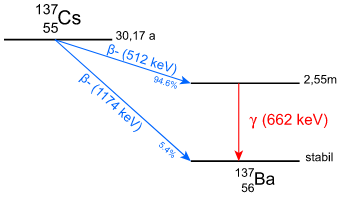
\includegraphics[scale=0.6]{content/schema.png}
    \caption{Zerfallschema von $\ce{^{137}Cs}$ \cite{leifi}.}
    \label{fig:schema}
\end{figure}
\vspace{-5pt}

Die emittierte Gammastrahlung kann über drei verschiedene Effekte mit Materie
wechselwirken:

\begin{itemize}
    \item Photoeffekt: Gammaquanten stoßen Hüllenelektronen aus deren Schalen durch Übertragung ihrer gesamten Energie $E_\gamma$,
    welche die Austrittsarbeit $W_e$ der Elektronen übersteigt ($E_\gamma > W_e$).
    \item Compton-Effekt: Gammaquanten streuen inelastisch an Elektronen und übertragen nur einen Teil ihrer Energie.
    \item Paarbildung: Gammaquanten zerfallen in den Coulomb-Feldern der Atome in Elektron-Positron-Paare. Dadurch
    wird ein Teil der Photoenergie in Ruheenergie gewandelt, die mindestens $2 m_e c^2 = \SI{1.02}{\mega\eV}$ beträgt.
\end{itemize}

Abhängig von der Photonenenergie $E_\gamma$ der Gammaquanten dominieren verschiedene dieser Effekte. 
Für kleine Energien mit $E_\gamma \leq \SI{100}{\kilo\eV}$ dominiert der Photoeffekt und für
mittlere Energien im Intervall $\SI{100}{\kilo\eV} \leq E_\gamma \leq \SI{1}{\mega\eV}$ ist der Compton-Effekt ausschlaggebend.
Für höhere Energien würde die Paarbildung dominieren, jedoch ist die Strahlung des $\ce{^{137}Cs}$ dafür nicht energiereich genug.

In einem in Abbildung \ref{fig:spektrum} dargestellten beispielhaften $\ce{^{137}Cs}$-Gammaspektrum kann man diese
Effekte auch an ihren Charakteristika erkennen. So kann man gut das Comptonspektrum mit Rückstreupeak beobachten, welches 
durch die Comptonkante abgeschlossen wird und dadurch klar vom Photo- bzw. Full Energy Peak unterscheidbar ist.
Dabei markiert die Comptonkante die maximale Energieabgabe der Gammaquanten durch Streueffekte an den Elektronen.
Am Photopeak wird die gesamte Energie der Gammaquanten vom Material absorbiert.

\vspace{-5pt}
\begin{figure}
    \centering
    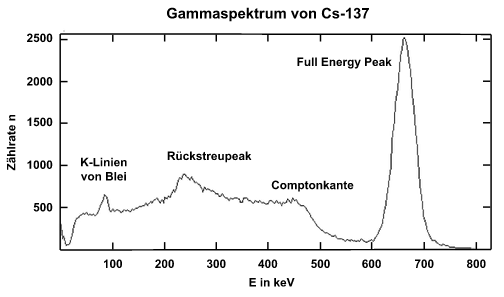
\includegraphics[scale=0.6]{content/spektrum.png}
    \vspace{-10pt}
    \caption{Gammaspektrum von $\ce{^{137}Cs}$ \cite{leifi}.}
    \label{fig:spektrum}
\end{figure}
\vspace{-5pt}

Für die Bestimmung der Absorptionkoeffizienten kann über eine Umformung der Gleichung \eqref{eqn:int}
die Matrixschreibweise erzielt werden

\begin{equation}
    \text{ln} \left(\frac{I_0}{I}\right) = \sum_i \mu_i d_i \qquad \to \qquad A \cdot \vec{\mu} = \vec{I} \; .
\end{equation}

Dabei setzt sich $\vec{\mu}$ aus allen Absorptionskoeffizienten der in der Probe vorliegenden Materialien zusammen
und $\vec{I}$ aus allen Anfangs- und abgeschwächten Intensitäten. Die $n \times m$-Matrix $A$ berücksichtigt die Schichtdicken
der verschiedenen Schnittgeometrien. 
Zur Anwendung der Methode der kleinsten wird eine Gewichtung 

\begin{equation}
    W \cdot A \cdot \vec{\mu} = W \cdot \vec{I} \:, \qquad W = Var[\vec{I}]^{-1}
\end{equation}

angwandt, wobei die Gewichtungsmatrix $W$ aus der Inversen der Kovarianzmatrix $Var[\vec{I}]$ gebildet wird.
Schließlich ergeben sich $\mu$ und dessen Unsicherheit $Var[\vec{\mu}]$ zu

\begin{equation}
    \vec{\mu} = \left(A^T \cdot W \cdot A\right)^{-1} A^T \cdot W \cdot \vec{I}\:, \qquad Var[\vec{\mu}] = \left(A^T \cdot W \cdot A\right)^{-1} \: .
    \label{eqn:Abs}
\end{equation}

